\documentclass[a4paper]{article}

\usepackage{fullpage} % Package to use full page
\usepackage{parskip} % Package to tweak paragraph skipping
\usepackage{tikz} % Package for drawing
\usepackage{amsmath}
\usepackage{hyperref}
\usepackage[utf8]{inputenc}
\usepackage{graphicx}
\usepackage{enumitem}
\usepackage{booktabs}
\usepackage{lmodern}
\usepackage[MeX]{polski}
\usepackage[T1]{fontenc}
\usepackage{float}
\usepackage{subfiles}

\title{Notatki z kursu Inżynieria Oprogramowania}
\author{Małgorzata Dymek}
\date{2018/19, semestr letni}

\begin{document}
    \maketitle

    \section{Podstawowe pojęcia}
    \subfile{podstawowe_pojecia}

    \section {UML}
    \subfile{uml}


    \section{Procesy wytwarzania oprogramowania}
    \subfile{procesy}


    \section{Standardy jakości}
    \subfile{standardy}

    \section{Zwinne procesy wytwarzania oprogramowania}
    \subfile{zwinne}


    \section{Wymagania}
    \subfile{wymagania}

    \section{Projektowanie systemu}
    \subfile{system}

    \section{Projektowanie obiektów}
    \subfile{obiekty}

    \section{Testowanie i kontrola jakości}
    \subfile{test}


    \section{Ewolucja oprogramowania i zarządzanie konfiguracją}
    \subfile{ewolucja}

    \section{Ciągła integracja, oprogramowanie w chmurze}

    \subsection{Ciągła integracja}
    Ciągła Integracja - praktyka polegająca na \textbf{jak najczęstszej integracji} zmian z istniejącym
    już systemem.

    \begin{table}[H]
        \begin{center}
            \begin{tabular}{ c p{6cm}}
                \raisebox{-\totalheight}{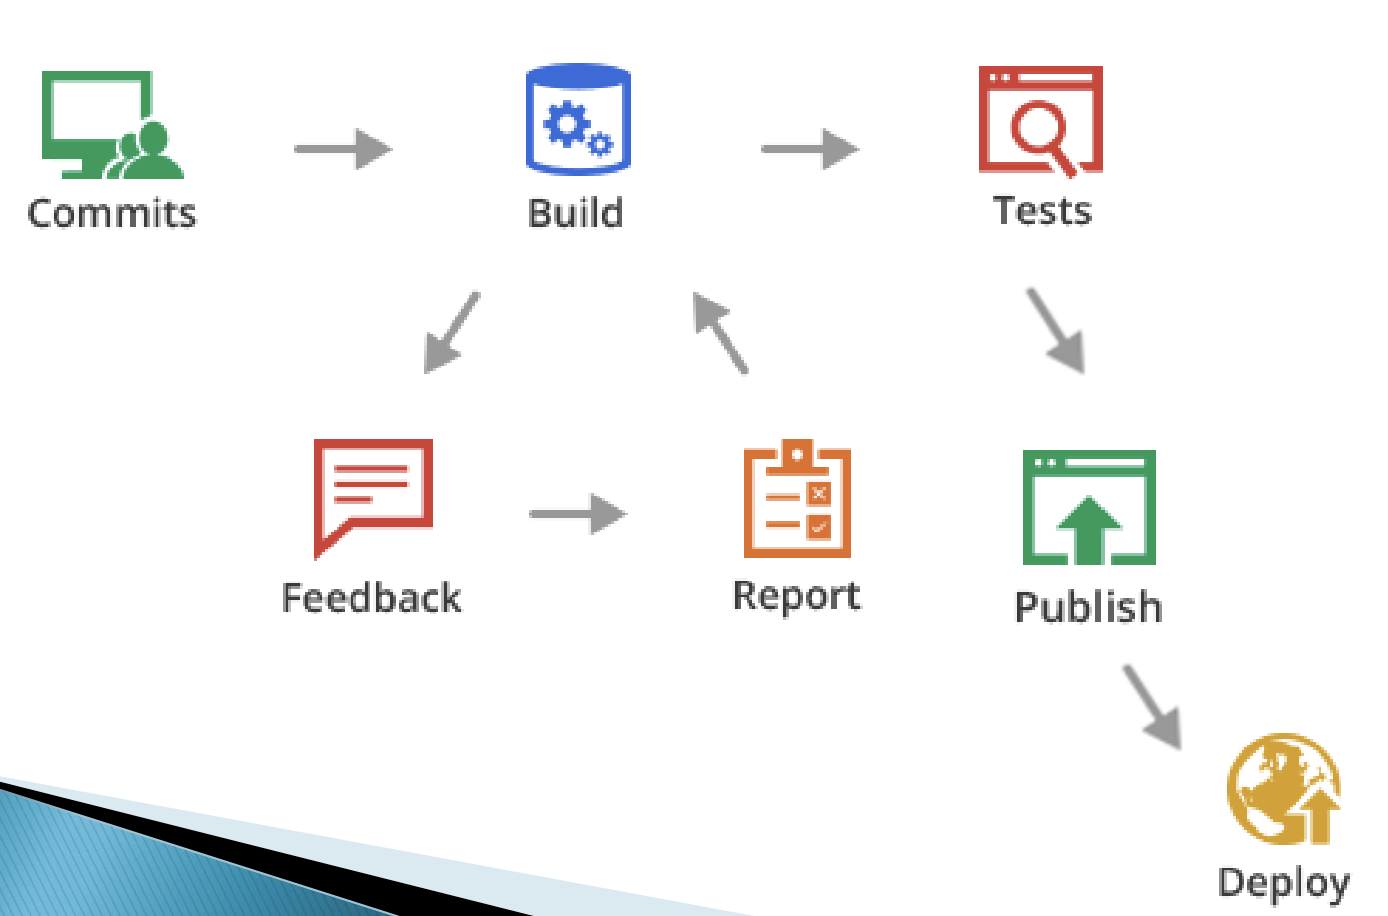
\includegraphics[width=0.5\textwidth]{integracja.png}}
                &
                \textbf{Zalety CI}
                \begin{itemize}
                    \item zmniejsza ilość pracy potrzebnej do łączenia zmian
                    z istniejącym kodem aplikacji.
                    \item wczesne wykrywanie konfliktów, błędów w
                    kompilacji i defektów w kodzie.
                    \item zawsze gotowa wersja demonstracyjna
                \end{itemize}
            \end{tabular}
        \end{center}
    \end{table}

    \textbf{Wymagania CI}
    \begin{itemize}
        \item repozytorium kodu
        \item skrypt umożliwiający automatyczne budowanie aplikacji
        \item Testy Jednostkowe
        \item wyzwalacz w postaci włącznika czasowego lub wykrywania zmiany w kodzie, albo połączenia obu.
        \item system powiadamiania o wynikach procesu i problemach
        \item zbiór wyników i interfejs dostępny dla każdego w dowolnym momencie
    \end{itemize}

    \subsection{Ciągłe dostarczanie oprogramowania}
    \begin{itemize}
        \item Za każdym razem, kiedy build pozytywnie przejdzie wszystkie testy, jest automatycznie wdrażany do
        środowiska testowego, gdzie można go poddać dalszym testom.
        \item Proces ten może nastąpić tylko raz, zanim oprogramowanie zostanie udostępniane klientom
        albo może się powtarzać, tworząc wiele nowych funkcji i poprawek zanim nadejdzie czas wydania.
    \end{itemize}


    \begin{figure}[H]
        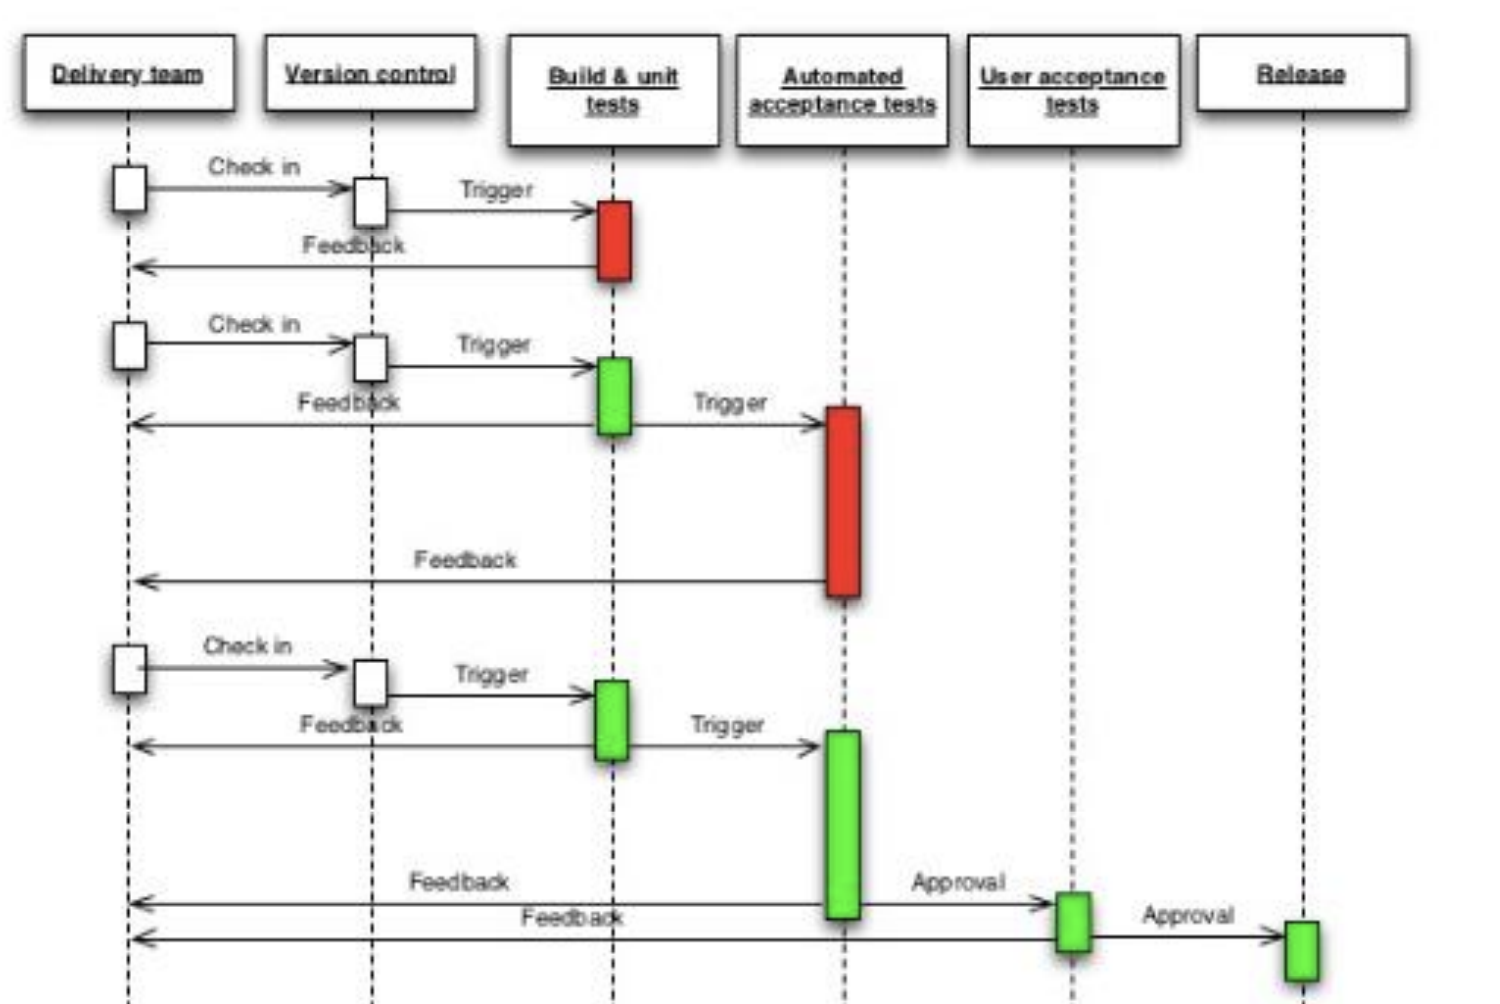
\includegraphics[width=\linewidth]{cdo.png}
    \end{figure}


    \subsection{Oprogramowanie w chmurze}
    Praca w chmurze obliczeniowej oznacza \textbf{pracę z aplikacjami lub usługami}, udostępnianymi przez
    internet.

    Praca odbywa się na \textbf{sieci serwerów} znajdujących się w centrum obliczeniowym.

    \begin{table}[H]
        \begin{center}
            \begin{tabular}{ p{.5\linewidth} p{.5\linewidth}}
                \textbf{Zalety} & \textbf{Wady}\\

                \begin{itemize}
                    \item Skalowalność
                    \item Dostępność
                    \item Wydajność
                    \item Łatwe zarządzanie
                    \item Elastyczność
                    \item Niezawodność
                    \item Ekologia
                \end{itemize}
                &
                \begin{itemize}
                    \item Bezpieczeństwo
                    \item Ograniczone rozwiązania
                    \item Wydajność
                \end{itemize}
            \end{tabular}
        \end{center}
    \end{table}



    \subsubsection{Modele dystrybucji}

    \begin{table}[H]
        \begin{center}
            \begin{tabular}{ p{.4\linewidth} p{.6\linewidth}}
                \textbf{Software as a Service - SaaS}
                &
                aplikacja jest przechowywana i wykonywana na
                komputerach dostawcy usługi i jest udostępniana
                użytkownikom przez Internet.
                \\

                \cmidrule(r){1-1}\cmidrule(l){2-2}
                \textbf{Infrastracture as a Service - IaaS}
                &
                polega na dostarczeniu przez dostawcę całej infrastruktury
                informatycznej, takiej jak np. wirtualizowany sprzęt,
                skalowany w zależności od potrzeb użytkownika.
                \\

                \cmidrule(r){1-1}\cmidrule(l){2-2}
                \textbf{Platform as a Service - PaaS}
                &
                polega na udostępnieniu przez dostawcę wirtualnego
                środowiska pracy; skierowana jest przede wszystkim do
                programistow.
                \\
            \end{tabular}
        \end{center}
    \end{table}



\end{document}

